\documentclass{beamer}

\usepackage{graphicx}
\usepackage{booktabs}
\usepackage[french]{babel}
%  \usepackage[T1]{fontenc}
%  \usepackage[latin1]{inputenc}
\usepackage{algorithm2e}

\mode<presentation> {
	% \usetheme{default}
	% \usetheme{AnnArbor}
	% \usetheme{Antibes}
	% \usetheme{Bergen}
	% \usetheme{Berkeley}
	% \usetheme{Berlin}
	% \usetheme{Boadilla}
	% \usetheme{CambridgeUS}
	% \usetheme{Copenhagen}
	% \usetheme{Darmstadt}
	% \usetheme{Dresden}
	% \usetheme{Frankfurt}
	% \usetheme{Goettingen}
	% \usetheme{Hannover}
	% \usetheme{Ilmenau}
	% \usetheme{JuanLesPins}
	% \usetheme{Luebeck}
	\usetheme{Madrid}
	% \usetheme{Malmoe}
	% \usetheme{Marburg}
	% \usetheme{Montpellier}
	% \usetheme{PaloAlto}
	% \usetheme{Pittsburgh}
	% \usetheme{Rochester}
	% \usetheme{Singapore}
	% \usetheme{Szeged}
	% \usetheme{Warsaw}

	% \usecolortheme{albatross}
	% \usecolortheme{beaver}
	% \usecolortheme{beetle}
	% \usecolortheme{crane}
	% \usecolortheme{dolphin}
	% \usecolortheme{dove}
	% \usecolortheme{fly}
	% \usecolortheme{lily}
	% \usecolortheme{orchid}
	% \usecolortheme{rose}
	% \usecolortheme{seagull}
	% \usecolortheme{seahorse}
	% \usecolortheme{whale}
	% \usecolortheme{wolverine}

	% \setbeamertemplate{footline} % To remove the footer line in all slides uncomment this line
	% \setbeamertemplate{footline}[page number] % To replace the footer line in all slides with a simple slide count uncomment this line
	\setbeamertemplate{navigation symbols}{} % To remove the navigation symbols from the bottom of all slides uncomment this line
}

\AtBeginSection[]{
	\begin{frame}
		\frametitle{Table des matières}
		\tableofcontents[currentsection]
	\end{frame}
}
\AtBeginSubsection[]{
	\begin{frame}
		\frametitle{Table des matières}
		\tableofcontents[currentsubsection]
	\end{frame}
}

\title[Audit]{Plate-forme d'entrainement de gestion de crise}
\author{Brandon Alves}
\institute[INSA Lyon]{
	INSA Lyon \\
	\medskip
	INRIA
}
\date{14 Juin 2021 - 13 Août 2021}

\begin{document}
	\begin{frame}
		\titlepage
	\end{frame}
	\begin{frame}
		\frametitle{Table des matières}
		\tableofcontents
	\end{frame}
	\section{Architecture du SI}
		\begin{frame}
			\frametitle{Architecture du SI}
			\begin{block}{Clients}
				\begin{itemize}
					\item debian-client1 (Debian 10)
					\item debian-client2 (Debian 10) : machine du patron
				\end{itemize}
			\end{block}
			\begin{block}{Serveurs}
				\begin{itemize}
					\item debian-web (Debian 9)
					\begin{itemize}
						\item dans DMZ
						\item LAMP
					\end{itemize}
					\item debian-mail (Debian 9)
					\begin{itemize}
						\item Poste.io
					\end{itemize}
					\item debian-dns (Debian 9)
					\begin{itemize}
						\item BIND9
					\end{itemize}
					\item debian-file (Debian 9)
				\end{itemize}
			\end{block}
		\end{frame}
		\begin{frame}
			\frametitle{Architecture du SI}
			\begin{block}{Routeur}
				\begin{itemize}
					\item pfsense (Freebsd)
					\item 5 interfaces (WAN, administration, dmz, clients, services)
					\item Firewall pfSense
					\item DHCP
				\end{itemize}
			\end{block}
			\begin{block}{Attaquant}
				\begin{itemize}
					\item debian-attacker (Debian 9)
					\item dans le réseau local de la machine roulant VirtualBox
					\item dispose de scripts ainsi que d'une interface web permettant de lancer différentes attaques
				\end{itemize}
			\end{block}
			\begin{block}{Administrateur}
				\begin{itemize}
					\item debian-admin (Debian 10) : machine de l'administrateur
				\end{itemize}
			\end{block}
		\end{frame}
		\begin{frame}
			\frametitle{Architecture du SI}
			\begin{center}
				\begin{figure}
					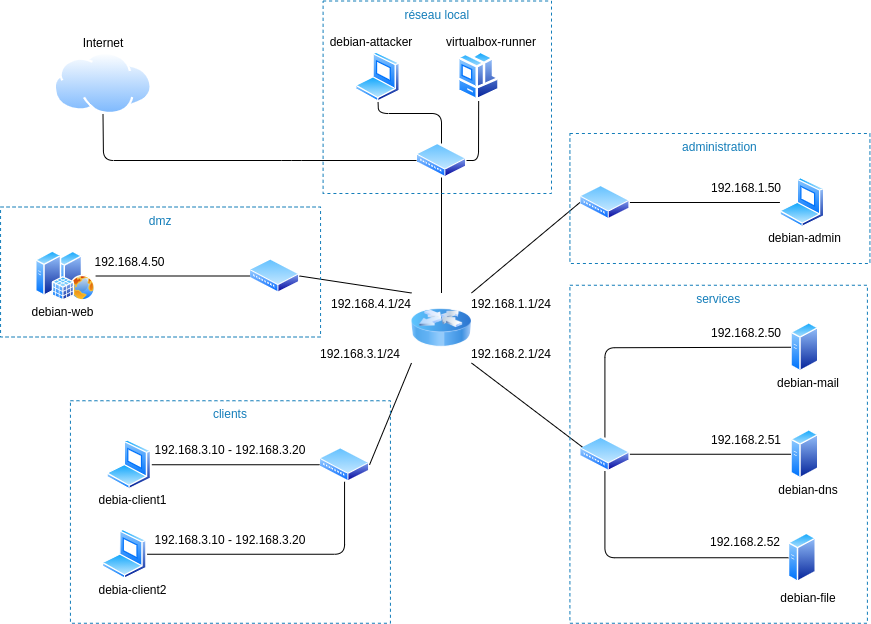
\includegraphics[scale=.3]{si.png}
					\caption{Architecture du SI}
				\end{figure}
			\end{center}
		\end{frame}
		\begin{frame}
			\frametitle{Déploiement de la plate-forme}
			\framesubtitle{Hébergement vs local}
			\begin{block}{Hébergement}
				\begin{itemize}
					\item Hébergé sur un serveur de l'INRIA;
					\item Connexion via \textit{Bureau à distance};
					\item Dépendant du réseau internet entre les machines et le serveur;
					\item Puissance de calcul plus élevée;
					\item Pas de conflit entre les différnetes cellules de crises.
				\end{itemize}
			\end{block}
			\begin{block}{Local}
				\begin{itemize}
					\item Indépendant du réseau internet entre les machines et le serveur;
					\item Difficile de faire tourner plus d'une cellule de crise sur un laptop.
				\end{itemize}
			\end{block}
		\end{frame}
	\section{Vulnérabilités \& Attaques}
		\begin{frame}
			\frametitle{Vulnérabilités \& Attaques}
			Vulnérabilités :
			\begin{itemize}
				\item Tout les comptes utilisateurs ont des mots de passe faibles;
				\item Tout les comptes mails ont des mots de passe faibles;
				\item RFI : vulnérabilité propre à Apache2;
				\item Aucun backup;
				\item Ancun filtre contre les spams mis en place;
				\item Firewall très permissif.
			\end{itemize}
		\end{frame}
		\begin{frame}
			\frametitle{Vulnérabilités \& Attaques}
			\begin{block}{Attaque SSH par force brute}
				Script qui tente de se connecter en SSH à la passerelle avec un nom d'utilisateur et un mot de passe contenue dans une liste de mots de passe les plus fréquant.
				Lorsqu'une combinaison pemet d'établir la connexion, celle ci est enregistrée dans un fichier.
			\end{block}
			\begin{block}{Attaque par déni de service (\textit{Slowloris})}
				Script qui envoie des requêtes HTTP partielles au serveur web, à intervalle régulier, afin de garder ses sockets ouverts.
			\end{block}
			\begin{block}{Attaque par déni de service (\textit{Ping})}
				Script qui envoie des pings (requêtes ICMP) au serveur web à intervalle régulier obligeant celui ci à répondre.
			\end{block}
		\end{frame}
		\begin{frame}
			\frametitle{Vulnérabilités \& Attaques}
			\begin{block}{Attaque par déni de service (\textit{UDP Flood})}
				Script qui envoie un large nombre de paquets UDP à la passerelle à des ports aléatoires.
				Le serveur doit alors vérifier qu'une application est en train d'écouter ou non sur ce port et répondre avec des paquets ICMP.
			\end{block}
			\begin{block}{Attaque par déni de service (\textit{TCP SYN Flood})}
				Script qui envoie une succession de requêtes SYN vers la cible, initialisant une connexion (three-way handshake).
				N'envoie pas le ACK final obligeant la cible a attendre un certain délais avant de fermer la connexion.
			\end{block}
			\begin{block}{Défacement de site web}
				Script qui utilise une vulnérabilité RFI (Remote FIle Inclusion). Utilise le programme \textit{weevely} pour se connecter au serveur.
			\end{block}
		\end{frame}
		\begin{frame}
			\frametitle{Vulnérabilités \& Attaques}
			\begin{block}{Phishing}
				Script qui envoie des mails aux différents utilisateurs. Le mail demande de se connecter à un site en entrant ses identifiants. L'attaquant récupère ces derniers.
			\end{block}
			\begin{block}{Ransomware}
				Script qui crypte le disque de la vm \textit{debian-file}.
			\end{block}
			\begin{block}{Spam (mail)}
				Script qui permet de spamer les différents utilisateurs par mail.
			\end{block}
			\begin{block}{Spam (blog)}
				Script qui permet de spammer sur le blog de l'entreprise.
			\end{block}
		\end{frame}
	\section{Informations}
		\begin{frame}
			\frametitle{Comptes utilisateurs 1/2}
			\begin{alertblock}{Sur \textit{debian-web}, \textit{debian-dns}, \textit{debian-mail}, \textit{debian-file}, \textit{debian-admin}, \textit{debian-client1} :}
				\begin{description}
					\item[login] admin
					\item[password] password
				\end{description}
			\end{alertblock}
			\begin{alertblock}{Sur \textit{debian-client1} :}
				\begin{columns}
					\begin{column}{.28\linewidth}
						\begin{description}
							\item[login] mcurie
							\item[password] fleur
						\end{description}
					\end{column}
					\begin{column}{.29\linewidth}
						\begin{description}
							\item[login] lpasteur
							\item[password] 12345
						\end{description}
					\end{column}
					\begin{column}{.34\linewidth}
						\begin{description}
							\item[login] hpoincare
							\item[password] motdepasse
						\end{description}
					\end{column}
				\end{columns}
			\end{alertblock}
			\begin{alertblock}{Sur \textit{debian-client2} :}
				\begin{description}
					\item[login] pdupont
					\item[password] argent
				\end{description}
			\end{alertblock}
		\end{frame}
		\begin{frame}
			\frametitle{Comptes utilisateurs 2/2}
			\begin{alertblock}{Sur \textit{debian-attacker} :}
				\begin{description}
					\item[login] attacker
					\item[password] password
				\end{description}
			\end{alertblock}
		\end{frame}
		\begin{frame}
			\frametitle{Mails utilisateurs 1/2}
			\begin{alertblock}{admin :}
				\begin{description}
					\item[login] admin@frenchleather.fr
					\item[password] password
				\end{description}
			\end{alertblock}
			\begin{alertblock}{pdupont :}
				\begin{description}
					\item[login] pierre.dupont@frenchleather.fr
					\item[password] argent
				\end{description}
			\end{alertblock}
			\begin{alertblock}{contact :}
				\begin{description}
					\item[login] contact@frenchleather.fr
					\item[password] contact
				\end{description}
			\end{alertblock}
		\end{frame}
		\begin{frame}
			\frametitle{Mails utilisateurs 2/2}
			\begin{alertblock}{mcurie :}
				\begin{description}
					\item[login] marie.curie@frenchleather.fr
					\item[password] fleur
				\end{description}
			\end{alertblock}
			\begin{alertblock}{lpasteur :}
				\begin{description}
					\item[login] louis.pasteur@frenchleather.fr
					\item[password] 12345
				\end{description}
			\end{alertblock}
			\begin{alertblock}{hpoincare :}
				\begin{description}
					\item[login] henri.poincare@frenchleather.fr
					\item[password] motdepasse
				\end{description}
			\end{alertblock}
		\end{frame}
		\begin{frame}
			\frametitle{SSH}
			Depuis l'extérieur, le SI est accessible via le protocole SSH sur la machine \textit{debian-file} et la machine \textit{debian-web}.
		\end{frame}
		\begin{frame}
			\frametitle{Web}
			Le site internet de l'entreprise est accessible à l'url : \url{http://www.frenchleather.fr}
		\end{frame}
		\begin{frame}
			\frametitle{Messagerie}
			Une interface web de messagerie est disponnible à l'url : \url{http://mail.frenchleather.fr}
		\end{frame}
		\begin{frame}
			\frametitle{Twitter}
			\begin{alertblock}{FrenchLeather - Connexion avec Google}
				\begin{description}
					\item[login] frenchleathersa@gmail.com
					\item[password] password123+
				\end{description}
			\end{alertblock}
			\begin{alertblock}{Attaquant - Connexion avec Google}
				\begin{description}
					\item[login] attacker554@gmail.com
					\item[password] 123password+
				\end{description}
			\end{alertblock}
		\end{frame}
		\begin{frame}
			\frametitle{Outils de monitoring du SI}
			Un tableau de bord est accessible à l'adresse \url{http://192.168.1.1} (login: \textit{admin}, password: \textit{password}).

			Différents outils de monitoring :
			\begin{itemize}
				\item état des différentes interfaces;
				\item informations générales sur l'état du routeur;
				\item status des différnts services du routeur;
				\item statistiques sur les interfaces;
				\item graphes représentant le traffic au niveau des interfaces;
				\item pfTop : différentes connexions établies;
				\item ...
			\end{itemize}
		\end{frame}
		\begin{frame}
			\frametitle{Firewall : règles}
			\url{http://192.168.1.1/firewall_rules.php}
			\begin{center}
				\begin{figure}
					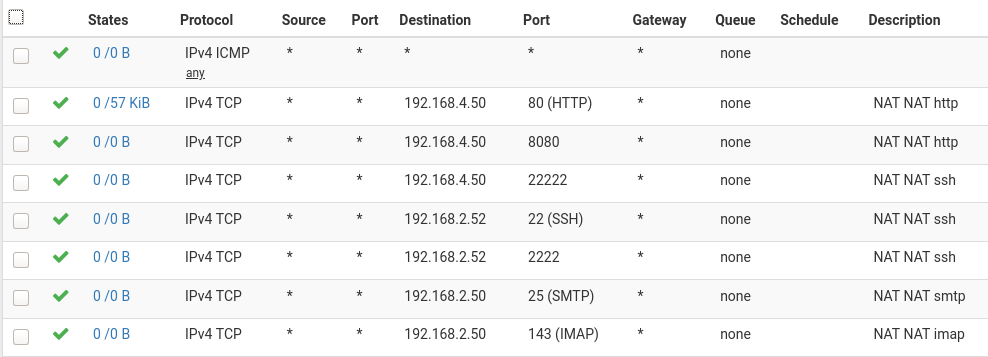
\includegraphics[scale=.3]{rule.png}
					\caption{Règles filtrantes du firewall}
				\end{figure}
			\end{center}
		\end{frame}
		\begin{frame}
			\frametitle{Firewall : NAT}
			\url{http://192.168.1.1/firewall_nat.php}
			\begin{center}
				\begin{figure}
					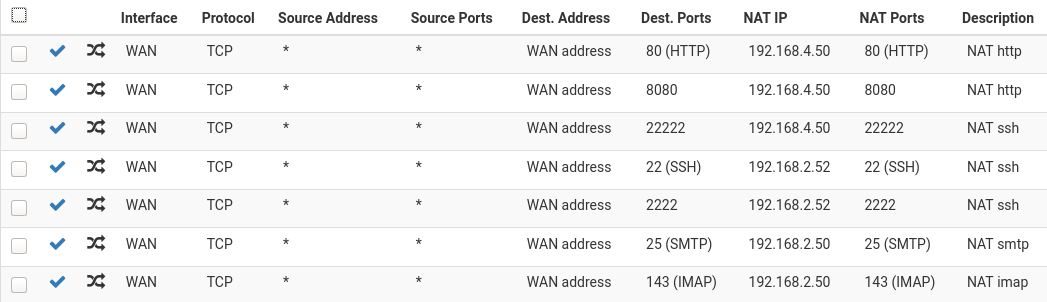
\includegraphics[scale=.3]{nat.png}
					\caption{Translations du firewall}
				\end{figure}
			\end{center}
		\end{frame}
		\begin{frame}
			\frametitle{Enregistrements DNS}
			$\$$ORIGIN frenchleather.fr.
			\begin{center}
				\begin{table}[h!]
					\centering
					\begin{tabular}{||c c c||}
						\hline
						Input & Type & Output \\
						\hline\hline
						 & SOA & debian-dns admin \\
						 & NS & debian-dns \\
						 & MX & 10 debian-mail \\
						debian-admin & A & 192.168.1.50 \\
						debina-dns & A & 192.168.2.51 \\
						debian-mail & A & 192.168.2.50 \\
						debian-web & A & 192.168.4.50 \\
						www & CNAME & debian-web \\
						mail & CNAME & debian-mail \\
						file & CNAME & debian-file \\
						ns & CNAME & debian-dns \\
						\hline
					\end{tabular}
					\caption{Enregistrements DNS}
					\label{table:1}
					\end{table}
			\end{center}
		\end{frame}
		\begin{frame}
			\frametitle{Pfsense}
			\url{http://192.168.1.1/}
			\begin{center}
				\begin{figure}
					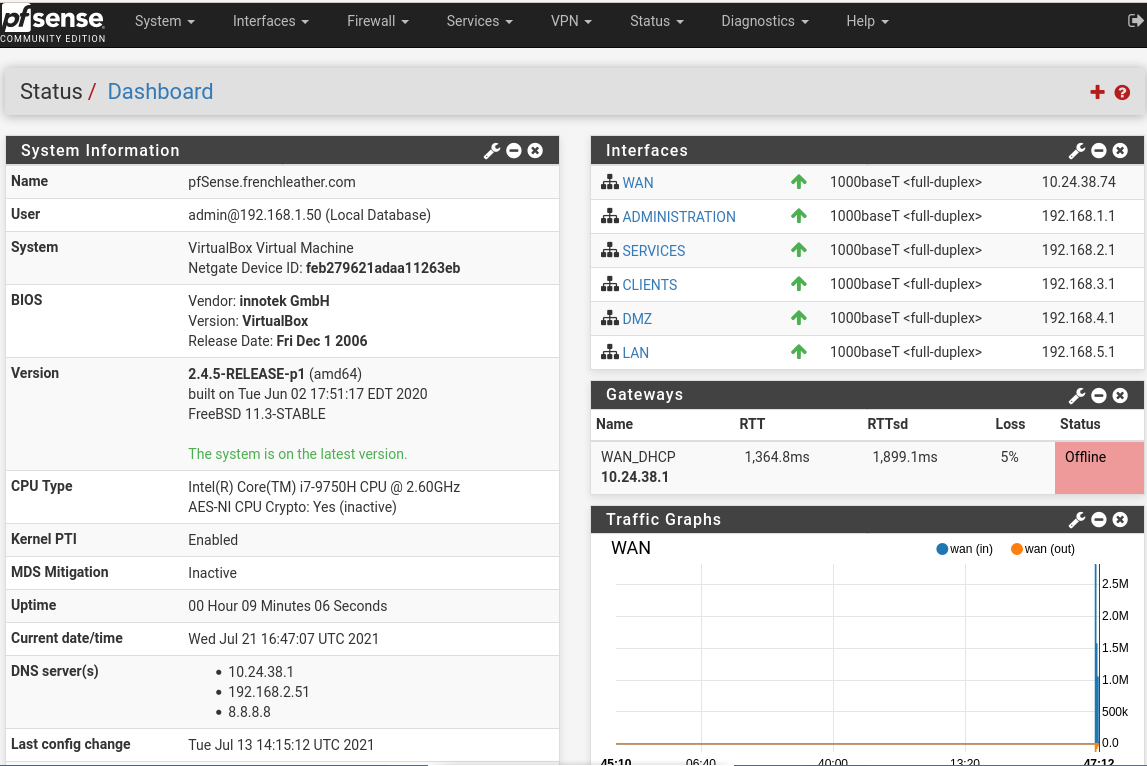
\includegraphics[scale=.22]{pfsense.png}
					\caption{Interface du routeur}
				\end{figure}
			\end{center}
		\end{frame}
		\begin{frame}
			\frametitle{Rspamd}
			\url{https://mail.frenchleather.fr/admin/rspamd/}
			\begin{center}
				\begin{figure}
					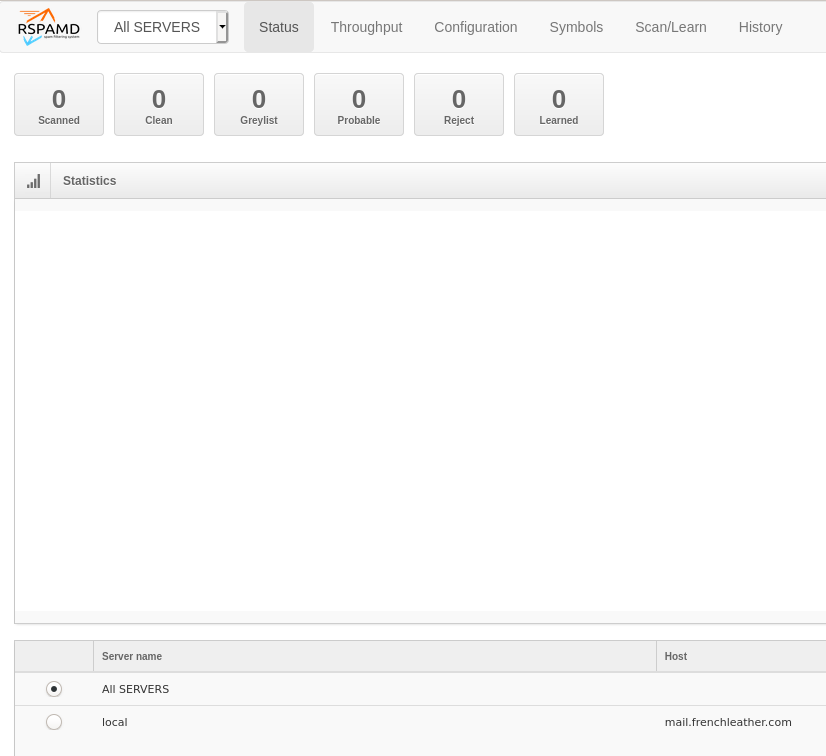
\includegraphics[scale=.23]{rspamd.png}
					\caption{Interface de l'antispam mail}
				\end{figure}
			\end{center}
		\end{frame}
		\begin{frame}
			\frametitle{Site web de l'entreprise}
			\url{http://www.frenchleather.fr/}
			\begin{center}
				\begin{figure}
					
\includegraphics[scale=.22]{www.png}
					\caption{Page d'accueil du site de l'entreprise}
				\end{figure}
			\end{center}
		\end{frame}
		\begin{frame}
			\frametitle{Interface de l'attaquant}
			\url{http://<adresse_IP_de_la_machine_attaquante>/}
			\begin{center}
				\begin{figure}
					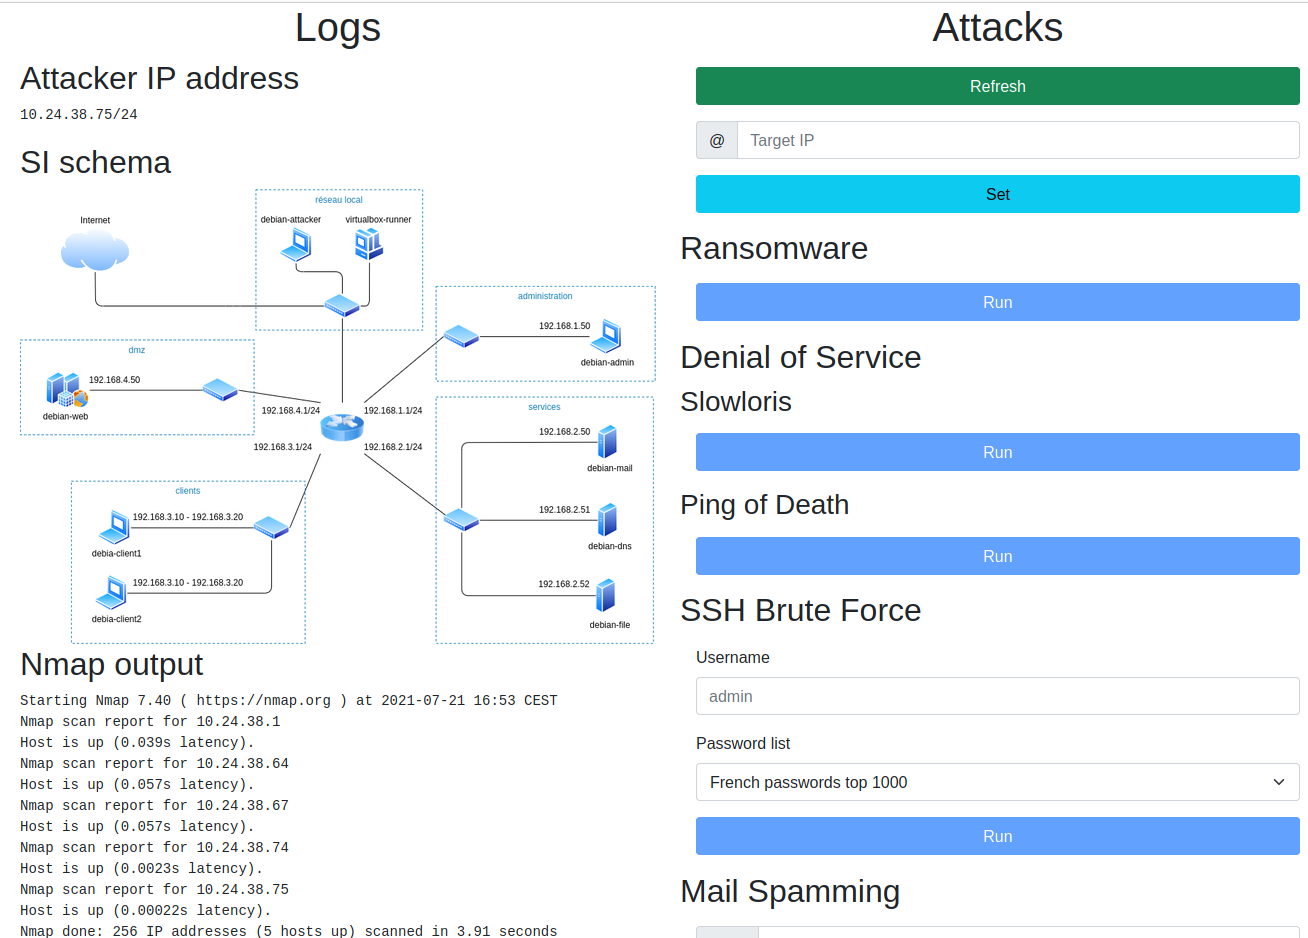
\includegraphics[scale=.18]{attacker.png}
					\caption{Interface de l'attaquant}
				\end{figure}
			\end{center}
		\end{frame}
		\begin{frame}
			\frametitle{Outils d'aide au controle des participants}
			\begin{itemize}
				\item Sur chaque machine, les commandes tapées sont enregistrées dans \url{/home/admin/.history/history.txt};
				\item Pour le firewall, on peut voir sur l'interface web du routeur ce qui a été modifié;
				\item Mesure du temps durant lequel le site web de l'entreprise est resté défacé;
				\item Mesure du temps durant lequel le temps de réponse à une requête au site web est trop long (pour le DoS);
				\item Nombres d'identifiant de connexions découverts (par l'attaque SSH ou phishing)
			\end{itemize}
		\end{frame}
\end{document}
